\cotefile{31}
\scanpage{87}

\uline{N.B.} Pour les bons anneaux locaux
henséliens de \deleted{\unsure{dim.}} car. résiduelle nulle, tout
est vérifié grâce à Artin.

% archive sheet number: 86
\scanpage{88}

\deleted{$G'=G_{S'}$ soit diagonalisable, i.e. de la forme $D_{S'}(M)$. Il est immédiat
qu'on peut se ramener au cas des $G'$, donc on peut supposer $G$ diagonalisable, donc il provient du groupe absolu $D_{\underline{Z}}(M)$ sur $\mathrm{Spec}(\underline{Z})$ par changement de base $S\quad\mathrm{Spec}(\underline{Z})$. Il suffit maintenant de conjuguer a) et 4.4.}

\deleted{\uline{Corollaire} 4.\handwritten{\unsure{8|7|9}}. \quad a) Soient $u,v:H\quad G$ deux homomorphismes de $S$-préschémas en groupes, avec $H$ diagonalisable de type fini, et \unsure{supposons|supposon} que pour tout entier $n\quad 0$, les restrictions de $u$ et $v$ à $ {}_nH$ sont identiques,. Alors $u\unsure{=}v$. \quad b) Soient $H_1,H_2$ deux sous-groupes de type multiplicatif et de type fini d'un préschéma en groupes $G$, et supposons que pour tout entier $n\quad 0$, on ait $ {}_nH_1=\deleted{\unsure{n}}{}_nH_2$, alors $H_1=H_2$.}

\deleted{La première assertion résulte de la seconde, par considération des
sous-groupes $H_1,H_2$ de $H\mathbin{\mathrm{x}}G$ graphes de $u$ et $v$. Pour prouver b), soit
$H=H_1\quad H_2$, c'est un sous-préschéma \inserted{en group\unsure{e|é}s} de \deleted{$H_1\unsure{H|M}$} $H_i$ $(i=1,2)$, il faut montrer qu'il est identique à $H_i$, or l'hypothèse signifie qu'il majore les $ {}_nH_i$. On est donc ramené à prouver le}

\deleted{\uline{Corollaire} 4.\handwritten{9}. \quad Soient $G$ un $S$-groupe de type multiplicatif et de type fini, et $H$ un sous-préschéma en groupes qui majore les $ {}_nG$, $n\quad 0$. Alors $H=G$.}

\deleted{En vertu de 4.6. on est ramené à prouver que le sous-préschéma
$\unsure{\mathbb H|H}$ est \uline{fermé}, ou encore qu'il est \deleted{\unsure{ident}} égal ensemblistement à $G$. Cela nous ramène au cas où $S$ est le spectre d'un corps, mais alors tout sous-préschéma en groupes de $G$ est fermé (Exp V), d'où la conclusion.}

\deleted{\uline{Remarque} 4.9. \quad Sous les conditions de 4.6., soit $m$ un entier $\quad 0$ qui a les propriétés suivantes: pour tout $s\quad S$, $m$ n'est pas \deleted{\unsure{la}} \inserted{une} puissance de la caractéristique de $k(s)$, et si $G_s$ est de type $M$, les diviseurs premiers de la torsion de $M$ divisent $m$. (NB cette deuxième condition}

% archive sheet number: 87
\scanpage{90}

\uline{Application} \quad Soit $X$ schéma projectif régulier sur
un corps $k$ \inserted{sép. clos}, $Y$ une section hyperplane
régulière, $F$ un faisceau de $l$-\deleted{\unsure{$l$|tor}}torsion loc.
constant sur $X$ \deleted{[$l$ premier à la car. de $k$]}.

On suppose \uline{$\dim X=n$}. Considérons $U=X-Y$ et

\diagram{\resizebox{\linewidth}{!}{\begin{tikzcd}[ampersand replacement=\&,column sep=small,row sep=1ex]
H^{i-1}(U,F)\arrow[r] \& H_Y^{\unsure{i|i-1}}(X,F)\arrow[r] \& H^i(X,F)\arrow[r] \& H^i(U,F)\arrow[r] \& H_Y^{i+1}(X,F)\\
\& \rotatebox{90}{$\simeq$} \& \& \& \rotatebox{90}{$\simeq$}\\
\& H^{i-2}(Y,F_Y\otimes\check T_{\deleted{\unsure{Y|l|\ell}}}) \& \& \& H^{\unsure{i+1|i-1}}(Y,F_Y\otimes\check T_{\deleted{\unsure{N|l|\ell}}})
\end{tikzcd}}}

et utilisons le fait que

\[ H^i(U,F)=0 \quad\text{si } i>n \]

On trouve le

\uline{Th de Lefschetz}

% vertical emphasis rule at left
\[
\begin{aligned}
\smash{\rule[-3ex]{.4pt}{5.8ex}}\qquad&\deleted{\unsure{H^i_Y(X,F)}}\\
&H^{i-2}(Y,F_Y\otimes\check T_l)\longrightarrow H^i(X,F)
\end{aligned}
\]

est \uline{surjectif} si $i\geqn+1$, \uline{bijectif} si $i\geq n+2$

\uline{Corollaire} \quad Supposons $X$ \uline{connexe} \inserted{\uline{régulier}} de dim $n$,
\llap{\smash{\rule[-1.8ex]{.4pt}{4.2ex}}\hspace{.7em}}alors $H^{2n}(X,\mu_N^{\otimes n})\simeq\mathbb Z/N\mathbb Z$ pour tt
entier $N$ premier à la car.

% archive sheet number: 89
\scanpage{91}

\uline{Dém}. Récurrence sur $n$, pour \inserted{$n=0$ \unsure{trivial|connu},} $n=1$
c'est connu, pour $n\geq 2$, on a \deleted{\unsure{en}}
$2n\geq n+2$ d'où en vertu du \unsure{th} de
Lefschetz

\[
H^{2n}(X,\mu_N^{\otimes n})\simeq H^{2n-2}
\left(Y,\underset{\substack{\rotatebox{90}{$=$}\\ \mu_N^{\otimes(n-1)}}}{\underline{\mu_N^{\otimes n}\otimes\check T}}\right)
\]

O.K.

\uline{Corollaire 2} \quad (\uline{Moye}\uuline{nn}\uline{ant \unsure{dualité}})

\[ H^j(X,F)\longrightarrow H^j(Y,F) \quad\text{est} \]

injectif si $j\leq n-1$, bijectif si $j\leq n-2$

Résulte du th de Lefschetz par
simple \uline{transposition}, à valeurs dans $\mathbb Q/\mathbb Z$.

% archive sheet number: 90
\scanpage{92}

\uline{Théorème de} \uline{Spécialisation}:

\margin{\unsure{9 p}}

Corollaire

% archive sheet number: 91
\scanpage{93}

\uline{Lemme 1} \quad $A$ anneau local noeth. \deleted{\unsure{quasi de}} \inserted{\deleted{\unsure{par hyp. un régulier}} quotient d'un régulier}
\deleted{formellement normal}, $t\in\unsure{\mathfrak r|r|\mathfrak m} A$ \inserted{un \unsure{élémt|élément} $A$-régulier}, on suppose
\deleted{$A/tA$ formellement normal} \inserted{le complété $t$-adique de $A$ normal} (à fortiori
$A$ \deleted{formellement} normal), et
$\dim A\geq 3$. Soit \deleted{$B$ fini sur $A$},
$B$ ``extension'' \inserted{finie} \uline{normale} \deleted{\unsure{génér.|de}} de $A$, et
supposons que $B/tB$ sur $A/tA$ soit
un rev. \deleted{\unsure{étale dans} le complément de l'origine} \inserted{\uline{trivial} hors de l'origine}.

\figure{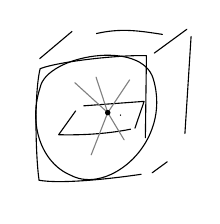
\begin{tikzpicture}[x=.27cm,y=.27cm,line cap=round,line join=round]
\draw (0,0) .. controls (-.15,1) and (-.25,4) .. (.05,5.25) .. controls (1,5.6) and (3.8,5.9) .. (5.05,5.86) -- (5,2);
\draw (0,0) .. controls (1,-.18) and (3.25,.05) .. (4.8,.28);
\draw (.03,5.72)--(1.55,7) (2.7,6.9)..controls(3.8,7.15)and(4.6,7.05)..(5.8,6.86) (5.42,5.98)--(6.95,7.1) (7.15,6.76)--(6.86,2.2) (5.32,.35)--(6.03,.87);
\draw (.92,2.14)--(1.72,3.26) (2.1,3.5)--(4.94,3.71)--(4.51,2.45) (4.3,2.4)..controls(2.7,2.08)and(1.2,2.14)..(.92,2.14);
\draw[gray] (3.23,3.18)--(1.68,4.59) (3.23,3.18)--(2.68,4.85) (3.23,3.18)--(4.26,4.72) (3.23,3.18)--(2.45,1.19) (3.23,3.18)--(4,1.9);
\fill (3.23,3.18) circle (.13); \fill (3.83,3.06) circle (.035);
\draw[thin] (.05,4.36) .. controls (.35,5.88) and (4.86,6.67) .. (5.38,4.74) .. controls (6.25,1.74) and (3.25,-.7) .. (1.5,.23) .. controls (.08,.82) and (-.51,2.68) .. (.05,4.36);
\end{tikzpicture}}

% slanted
\margin{Il suffit pour une \unsure{modification|rédaction|réduction} \unsure{minime|minima} de supposer que $B/tB$ coïncide dans le complémentaire de l'origine de $\unsure{\mathrm{Sp}}\,A/tA$ avec la restriction d'un rev. \uline{étale} de $A/tA$, \deleted{\unsure{ce dernier}} \deleted{\unsure{$A$}}}

Alors $B$ est un revêtement étale \deleted{hors de l'origine}

\uline{N.B.} L'hyp. implique que $B$ est étale sur $A$ en les pts de $V(t)-\text{origine}$ (grâce à la normalité de $A$ et $B$ \ldots\unsure{]|)} 

\deleted{Il revient \unsure{au même} de dire qu'il existe un}

\deleted{Comme} \deleted{Soit} $X=\mathrm{Spec}\,A$, \deleted{Soit} $X'=X-\{0\}$, $U$ l'ouvert des
pts de $\unsure{X|X'}$ en les quels $B$ est étale, alors
\deleted{[si $U\ne X$]} $(X-U)\cap V(t)\deleted{\unsure{=\varnothing}}\unsure{\subset|=}\{0\}$ et
$\dim(X-U)\leq 1$. On a un \unsure{revêtmt|revêtement} étale
\deleted{\unsure{de $X$}} \inserted{de} $U$, et il faut montrer qu'il se
prolonge en un rev. étale de $X$ \unsure{tt|\ensuremath{{}^{\prime}}}, \deleted{\unsure{un}}
\deleted{par le \unsure{compl.} dans les hyp. de} \deleted{\unsure{dim. et}}
Comme aux pts de $X-U$,
on a $\operatorname{prof}\mathscr O_{X,x}\geq 2$ [car $\dim\mathscr O_{X,x}\geq 2$,
et $\mathscr O_{X,x}$ est normal], cela signifie que

% slanted
\margin{condition des chaînes}

% archive sheet number: 92
\scanpage{94}

\mspage{(2)}

l'\unsure{algèbre} \rlap{\raisebox{-1.2ex}{\tikz{\draw[gray!45,thin] (0,0) ellipse (1.48em and 1.6ex);}}}$i_*(\mathscr A)$ sur $X$ est étale [$i:U\longrightarrow X$
imm. canonique, $\mathscr A$ l'Algèbre \inserted{sur $U$} \unsure{qui|que} définit
$V/U$]. Sous \unsure{cette} forme, l'énoncé est
invariant par \deleted{\unsure{un}} changmt de base fid plat
\unsure{qu.} \unsure{cpt|que} $X_1\longrightarrow X$, ce qui nous ramène
au cas où $A$ est \uline{complet} \deleted{\unsure{pour sa}} pour sa
\deleted{complété pour la top.} topologie $t$-adique.

% slanted
\margin{$A$ quotient d'un régulier, \deleted{ou $A/tA$ formellement normal} \uline{ou} $A/tA$ form. normal}

\deleted{Or dans ce cas De plus Or on a un isomorphisme des complétés}

Dans ce cas, nous allons prouver que en
fait, $B$ est un revêtement \uline{trivial} de $A$.

Or \deleted{\unsure{on}} \unsure{,} si $n$ est le \deleted{\unsure{degré|duplique}} \inserted{rg} de $B$ sur $A$,
il existe un isom \uline{formel} du
revêtement normal $Y'$ de $X'$ défini par $B$,
avec le rev. trivial $X'\times[1,n]$. Il
reste à prouver que c'est là un
isom régulier, et pour ceci il \deleted{\unsure{nous}}
faut vérifier que pour tt pt \uline{fermé}
$x$ de $X'$, \deleted{\unsure{$B$}} \rlap{\raisebox{-1ex}{\tikz{\draw[gray!30,thin] (0,0) ellipse (.9em and 1.5ex);}}}$\mathscr A_x$ est de prof $\geq 2$.

% slanted
\margin{\uline{SGA 1962}}

\uline{Or} \unsure{cela} résulte du fait que $A$
satisfait la condition des chaînes, et $B$
est une ``extension'' normale.

% archive sheet number: 93
\scanpage{95}

\uline{Lemme 2} \quad Soit $f:X\longrightarrow Y$ un morphisme
\llap{\smash{\rule[-13ex]{.4pt}{15ex}}\hspace{.65em}}\deleted{\unsure{de} simple} \inserted{lisse} à fibres de dim 1,
$g$ une section de $X$ sur $Y$, $Y$ \deleted{normal}
\deleted{loc.} \unsure{noeth|excllt} normal \inserted{intègre}, donc $X$ normal. Soit
$X'\longrightarrow X$ rev. normal galoisien de
groupe $\Gamma$ \deleted{premier \unsure{aux}} d'ordre premier aux
car. résiduelles de $Y$, \deleted{muni d'une
section de $g^{-1}($ --- tel que $g^{-1}(X')$
est une section naturelle. Alors \unsure{,}}

Supposons de plus \deleted{que qu'il existe
une partie fermée \inserted{\unsure{vraie}} $\unsure{D|Z|B}$ de $Y$, \unsure{un}
telle que $X$ soit étale sur $X-f^{-1}(Z)$.}

\deleted{[i.e. que la restriction de $X'$ à \unsure{?}
\deleted{fibre} \inserted{fibre gén} $X_{\unsure{\eta|y}}$ du \unsure{pt voisin} soit étale}

[($\eta$) étant le pt générique de $Y$] que
$X'_{\eta}$ sur $X_{\eta}$ soit étale, \deleted{en les pts de}
et que la fibre de $X'_{\eta}$ en $\xi=g(\eta)$ \deleted{soit}
\deleted{\unsure{comp}} ait un $p^{t}$ rat. sur $k(\xi)$ (ou
soit \unsure{complètemt} décomposé]. Alors $X'$ est
étale sur $X$ en les pts de $\unsure{g|s}(Y)$.

% archive sheet number: 94
\scanpage{96}

En vertu du Cor. au lemme 1, on est
ramené à prouver que en tt pt
\unsure{de} $x$ de $Y$ de codim 1 dans $Y$, \deleted{\unsure{on}}
$X'$ est \deleted{\unsure{non ramifié}} étale sur $X$ en les
$g(x)$. [N.B. Comme $X\unsure{-|\to}Y$ est
simple de dim relative 1, on notera
que $g(Y)$ est \deleted{défini loc. par} loc. un
diviseur de Cartier]. On est ainsi
ramené au cas où $Y$ est \deleted{le} spectre
d'un anneau de val. discrète, et \deleted{\unsure{qui}} on
est alors ramené [\unsure{en} examinant $\mathscr O_{X,g(x)}$]

% slanted
\margin{On a laissé tomber les conditions ``quotient d'un régulier'', c'est \unsure{loisible} en se ramenant aux alg. de type fini sur $\mathbb Z$\ldots}

\uline{Lemme 3} \quad Soit $A$ un anneau local
\uline{régulier} de dim $2$, $(x,y)$ un syst. régulier
de paramètres de $A$, $B$ une
``extension'' normale de $A$,
\deleted{\unsure{non ramifiée au pt}} \inserted{telle que}
\unsure{galoisienne|génériquemt}, (i) \deleted{de} groupe de Galois $\Gamma$
d'ordre premier à la car. résiduelle de $A$,
et telle que \deleted{\unsure{$B$ sur|$B\to$}} (ii) l'ens de ramification
de $B$ soit contenu dans $V(x)$ (iii)
le rev. se décompose complètemt en \deleted{$V(y)$}
le pt maximal $\unsure{y|\eta}$ de $V(y)$.

\figure{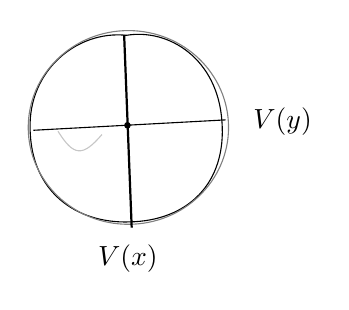
\begin{tikzpicture}[x=.6cm,y=.6cm]
\draw (0,1.95) .. controls (-1.05,2.06) and (-2.08,1.2) .. (-2.04,-.03) .. controls (-2.02,-1.38) and (-1.05,-2.03) .. (.05,-2) .. controls (1.31,-1.98) and (2.12,-1.17) .. (2.02,.13) .. controls (1.93,1.45) and (.9,2.1) .. (0,1.95);
\draw[thin,gray] (.04,0) ellipse (2.12 and 2.05);
\draw[thin,gray!45] (-1.45,-.08)..controls(-1.12,-.61)and(-.93,-.63)..(-.52,-.15);
\draw[line width=.8pt] (-.05,1.96)--(.11,-2.12);
\draw (-1.97,-.06)--(2.1,.16); \fill (.02,.045) circle (.07);
\node[right] at (2.48,.13) {$V(y)$}; \node[below] at (.03,-2.28) {$V(x)$};
\end{tikzpicture}}

% archive sheet number: 95
\scanpage{97}

Sous ces conditions, $B$ est étale sur $A$.

On peut supposer [quitte à faire une
\deleted{\unsure{extens.}} changmt de base $A'\unsure{-|\to} A$, $A'$ la
clôture \unsure{strictemt} locale de $A$] que $A$ est
\unsure{strictemt} local. \deleted{Alors il est \unsure{connu}} De plus
on peut supposer $B$ intègre. Alors il
est connu \inserted{(Abhyankar)}, grâce à (i) \inserted{(ii)}, que
$\Gamma=\mathbb Z/n\mathbb Z$, $B$ est de la forme $A[T]/(T^n-x)$.

% slanted
\margin{\uline{expliciter en} \uline{Lemme}}

Si $A'=A/yA$, alors $B\otimes_A A'=A'[T]/(T^n-x')$,
où $x'$ est l'image de $x$ dans $A'$, qui est un
uniformisant. On conclut \unsure{maintent|maintenant}
grâce à (iii).

% slanted
\margin{\deleted{N.B. On a laissé tomber dan\unsure{s}}}

\deleted{\unsure{Coroll.|Corollaire}} \uline{Théorème} \quad Soit \deleted{$A$ un anneau noeth.}
\deleted{$f:X\longrightarrow Y$ un morphisme essentiellement}
$f:X\longrightarrow Y$ un morphisme lisse,
\deleted{$Y$ loc. \unsure{noeth}}. Alors $f$ est loc.
1-asphérique pour les groupes finis
d'ordre premier aux car. résiduelles
de $Y$.

% archive sheet number: 96
\scanpage{98}

\uline{Dém} \quad On est ramené au cas où
$Y$ est \inserted{noeth} \unsure{strictemt|strictement} local, et par transitivité au cas
où $X$ est de dim relative 1 sur $Y$.\thinspace\ldots\thinspace.

\figure{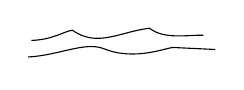
\begin{tikzpicture}[x=.5cm,y=.5cm]
\draw (0,0)..controls(.55,.02)and(.8,.22)..(1.04,.26)..controls(1.68,-.19)and(2.24,.22)..(3,.31)..controls(3.38,.01)and(4,.15)..(4.37,.13);
\draw (-.08,-.42)..controls(.7,-.38)and(1.36,-.02)..(1.84,-.21)..controls(2.65,-.54)and(3.47,-.16)..(3.62,-.18)--(4.67,-.23);
\end{tikzpicture}}

\uline{Applications} 1) Soit $f:X\longrightarrow Y$ un morphisme qu. cpt
\llap{\smash{\rule[-2.1ex]{.4pt}{4.6ex}}\hspace{.65em}}qu. sép. Alors les $R^i\unsure{f|f_*}(F)$ \unsure{commutent|hom. naturel|homomorphisme|localement constant} \unsure{à|:}
\unsure{tt|toute|par} extension lisse de la base.

\deleted{2) Soit $X$}

2) $X$ préschéma sur un corps sép. clos. Alors
pour $k'/k$ ext. sép. clos, et tt $F$ de
torsion sur $X$ premier \deleted{\unsure{à}} à car. de $k$, on
a

\[ H^i(X,F)\xrightarrow{\sim}H^i(X',F') \]

(Étendre au $H^1$ et $H^2$ non commutatifs \ldots)\unsure{.|,}

3) Si $X$ lisse sur $S$, $Y$ sous-schéma lisse,
calcul des $\underline H^i_Y(F)$, $F$ loc constant sur
$X$ premier aux car. résiduelles (\uline{th. de
pureté relatif}).

% archive sheet number: 97
\scanpage{99}

\uline{Corollaire} \quad Soit $Y$ un sous-schéma fermé
de $X$, \deleted{\unsure{fais.} --- \unsure{faisons les}} \deleted{\inserted{Soit $L'=\operatorname{Hom}(L,I_{X/S})$}} \deleted{Conditions
équivalentes}: $V=X-Y$, $g:Y\unsure{-|\to} S$ et
$h:\deleted{\unsure{\to}} V\longrightarrow S$ induits par $f$, Posons
$F'=\operatorname{Hom}(F,I_{X/S})$. Conditions équivalentes:

% slanted
\margin{On peut aussi donner des énoncés sans dualité, en introduisant les $\underline H^q_Y(F)$ et $R^p f_{Y\unsure{*|-}}(\underline H^q_Y(F))$\ldots}

% slanted
\margin{Donner le cas d'un ``morphisme élémentaire''\ldots}

\diagram{\begin{tikzcd}[ampersand replacement=\&,column sep=.35em,row sep=1ex]
{}\arrow[dd,bend right=65] \& \text{(ii)} \& \mathbb R^i \deleted{\unsure{f|g}}h_!(F'|V) \& \text{loc. constant pour tt } i\\
{} \& \text{(i)} \& \mathbb R^i \deleted{\unsure{g|f}}h_*(F|V) \& \rule{7em}{.3pt}\\
{} \& \text{(iii)} \& \mathbb R^i g_*(\deleted{F} F'|Y) \& \deleted{\text{loc.}}\ \rule{6em}{.3pt}
\end{tikzcd}}

Ces conditions sont vérifiées si
$Y$ est \deleted{\unsure{simple|lisse}} \inserted{lisse} sur $S$, [plus généralement
\deleted{\unsure{si} \unsure{c'est} \unsure{en}} \inserted{s'il est plat$/S$ et} à fibres n'ayant que des
singularités ``normal crossings??].

L'équivalence de (i) et (iii)
résulte de la suite exacte de cohomologie
associée à

\[ 0\longrightarrow F_{V,X}\longrightarrow F\longrightarrow F|Y\longrightarrow 0,\]

l'équivalence de (i) et (ii) résulte du
th. de dualité \deleted{pour} \unsure{les} (une fois
qu'on s'est ramené au cas $S$ \deleted{\unsure{str.}} spectre
d'un anneau de val. \unsure{discrète} str. hens.].

% archive sheet number: 98
\scanpage{100}

\mspage{VII - 9 -}

n\textsuperscript{o}339

tifs des éléments de $P(A)$.

Ainsi, pour $x\handwritten{\in}K^{\handwritten{*}}$, on définit des entiers rationnels $v_P(x)$ en posant

\begingroup\csname tagsleft@true\endcsname
\[ \operatorname{div}(x)=\handwritten{\sum}_{P\handwritten{\in}P(A)}v_P(x)\mathbin{.}P\ .\tag*{(3)} \]
\endgroup

Des relations $\operatorname{div}(xy)=\operatorname{div}(x)+\operatorname{div}(y)$ et $\operatorname{div}(x+y)\handwritten{\geq}\inf(\operatorname{div}(x),\operatorname{div}(y))$, on déduit que les $v_P$ sont des valuations discrètes. Pour que $x\handwritten{\in}A$, il faut et il suffit que $\operatorname{div}(x)\handwritten{\geq}0$, c'est à dire que $v_P(x)\handwritten{\geq}0$ pour tout $P\handwritten{\in}P(A)$. Ainsi les $v_P$ vérifient les conditions (AK.1) et (AK.2), et évidemment aussi (AK.3).

C.Q.F.D.

COROLLAIRE.- \uline{Pour qu'un anneau noethérien soit un anneau de Krull}, \uline{il faut et il suffit qu'il soit intégralement clos}.

En effet un anneau noethérien intégralement clos est complètement intégralement clos (Chap.V,\S1,n\textsuperscript{o}3).

4.- \uline{Valuations essentielles d'un anneau de Krull}.

Soit $A$ un anneau de Krull. Les éléments de $D(A)$ sont alors appelés les \uline{diviseurs} de $A$, et les classes de $D(A)$ suivant le sous-groupe des diviseurs principaux sont appelées les \uline{classes de diviseurs} de $A$. On appelle \uline{valuations essentielles} de $A$ les valuations $v_P$ définies, comme au n\textsuperscript{o} précédent, par la formule

\begingroup\csname tagsleft@true\endcsname
\[ \operatorname{div}(x)=\handwritten{\sum}_{P\handwritten{\in}P(A)}v_P(x)\mathbin{.}P\tag*{(4)} \]
\endgroup

pour $x\handwritten{\in} K^{\handwritten{*}}$. On a remarqué, au cours de la démonstration du th.1, que les valuations $v_P$ vérifient les propriétés (AK.1), (AK.2) et (AK.3) de la déf.2.
En outre, ces valuations discrètes $v_P$ sont \uline{normées} : en effet, pour tout diviseur extrémal $P\handwritten{\in}P(A)$, on \inserted{\handwritten{a}} $P\handwritten{<}2P$, donc, si $\underline a$ et $\underline b$ sont les idéaux divisoriels correspondant à $P$ et $2P$, on a $\underline a\handwritten{\supset}\underline b$ et $\underline a\handwritten{\ne}\underline b$ ; pour $x\handwritten{\in}\underline a-\underline b$, on a $\operatorname{div}(x)\handwritten{\geq}P$ et $\operatorname{div}(x)\handwritten{\unsure{\ngeq|\ne}}2P$, d'où $v_P(x)=1$, ce qui démontre notre assertion.

PROPOSITION 6.- \uline{Soient} $A$ \uline{un anneau de Krull}, $K$ \uline{son corps des fractions}, \uline{et}

% archive sheet number: 99
\scanpage{101}

\uline{N.B.} Il y aurait lieu d'examiner aussi la situation où
on a un faisceau loc. constant
$G$ \uline{sur $V$} \uline{seulement} [pas néc.
prolongeable à $X$], \deleted{\unsure{Du fait alors}} et qu'on
se propose d'étudier \inserted{les} $\mathbb R^i h_*(G)$.

On a une suite \deleted{\unsure{exacte}} spectrale

\[ \mathbb R^{\unsure{*|n|i}}\unsure{h_*|h}(G)\Longleftarrow \mathbb R^p f_*(\mathbb R^q i_*(G)) \]

où $i:V\unsure{-|\to}X$ est l'immersion.

Tout est bien si les $\mathbb R^p f_*(\mathbb R^q i_*(G))$
sont loc. constants. Le Pb. ne
semble pas facile, \inserted{même si $Y$ lisse$/S$,} à cause des
phénomènes de ``wild ramification''
qui peuvent se produire [si $\operatorname{codim}(Y,X)$
$\geq 2$, il n'y a pas d'ennui, car $G$
se \unsure{prolonge} alors en un faisceau
loc. constant \ldots\thinspace.]. \deleted{Peut-être \unsure{est}}

% archive sheet number: 100
\scanpage{102}

\mspage{VII - 7 -}

n\textsuperscript{o}339

3) Soient $F$ un corps, et $R_1,\ldots,R_n$ des sous-anneaux de $F$ qui soient des anneaux de Krull. Alors leur \uline{intersection} $S=\handwritten{\bigcap}_{j=1}^{n}R_j$ est un anneau de Krull.

En effet, pour $1\handwritten{\leq}j\handwritten{\leq}n$, soit $(v_{ji})_{i\handwritten{\in}I_j}$ une famille de valuations du corps des fractions de $R_j$ vérifiant (AK.1), (AK.2), (AK.3) (où $A$ est remplacé par $R_j$). Notons $w_{ji}$ la restriction de $v_{ji}$ au corps des fractions de $S$. Alors la famille $(v_{ji})_{1\handwritten{\leq}j\handwritten{\leq}n,\ i\handwritten{\in}I_j}$ vérifie évidemment (AK.2) (où $A$ est remplacé par $S$), et aussi (AK.3) puisque l'ensemble des indices $j$ est fini. Les valuations $w_{ji}$ sont, soit discrètes, soit impropres. En ne gardant que celles qui sont discrètes, on obtient évidemment une famille vérifiant (AK.1), (AK.2) et (AK.3) (où $A$ est remplacé par $S$). Donc $S$ est bien un anneau de Krull.

4) En particulier, si $A$ est un anneau de Krull et $K'$ un sous-corps du corps des fractions $K$ de $A$, $K'\handwritten{\cap}A$ est un anneau de Krull.

THEOREME 1.- \uline{Soit} $A$ \uline{un anneau \unsure{intégré|intégre|intègre}}. \uline{Pour que} $A$ \uline{soit un anneau de Krull il faut et il suffit que les deux conditions suivantes soient satisfaites} :

a) $A$ \uline{est complètement intégralement clos} ;

b) \uline{toute famille non vide d'idéaux entiers divisoriels de} $A$ \uline{admet un élément maximal}.

Soit $A$ un Anneau de Krull. Il est complètement intégralement clos (Chap.VI, \S4, n\textsuperscript{o}3, cor. de la prop.9). Soit $(v_i)_{i\handwritten{\in}I}$ une famille de valuations du corps des fractions $K$ de $A$ vérifiant (AK.1), (AK.2) et (AK.3). On peut supposer les $v_i$ normées. Pour tout $\underline a\handwritten{\in}I(A)$, nous poserons

\begingroup\csname tagsleft@true\endcsname
\[ v_i(\underline a)=\sup_{\underline a\handwritten{\subset}Ax}\,(v_i(x))\ ;\tag*{(2)} \]
\endgroup

on a $v_i(\underline a)\handwritten{\in}Z$, car, si $a$ est un élément non nul de $\underline a$, la relation $Ax\handwritten{\supset}Aa$ implique $v_i(x)\handwritten{\leq}v_i(a)$ (d'après (AK.2)), ce qui montre que la famille des $v_i(x)$ ($\underline a\handwritten{\subset}Ax$) est majorée. Etablissons les propriétés suivantes :

1) \uline{Soit} $\underline a$ \uline{un idéal divisoriel} ; \uline{pour que} $y\handwritten{\in}\underline a$, \uline{il faut et il suffit que}

% archive sheet number: 101
